% Q3 summarization section

\subsection{Problem Formulation}
We study text summarization on CNN/DailyMail and compare extractive methods (selecting sentences) against abstractive methods (generating new text). Given an article $x$, the system outputs a summary $\hat{y}$ that should be fluent, faithful to the source, and cover the main points. We evaluate with ROUGE, BLEU, METEOR, and BERTScore.

\subsection{Dataset Description}
CNN/DailyMail \citep{Hermann2015cnndm} (version 3.0.0) provides news articles with reference highlights. We use a subset for tractable computation.

\begin{table}[H]
\centering
\caption{CNN/DailyMail dataset statistics.}
\begin{tabular}{lrr}
\toprule
\textbf{Split} & \textbf{Original Size} & \textbf{Subset Size} \\
\midrule
Train & 287,113 & 10,000 \\
Validation & 13,368 & 1,000 \\
Test & 11,490 & 1,000 \\
\bottomrule
\end{tabular}
\end{table}

\begin{table}[H]
\centering
\caption{Average document statistics (computed on test subset).}
\begin{tabular}{lrrrr}
\toprule
\textbf{Avg Article Len (words)} & \textbf{Avg Summary Len (words)} & \textbf{Avg Sentences} & \textbf{Compression Ratio} \\
\midrule
676.08 & 55.21 & 32.91 & 12.25 \\
\bottomrule
\end{tabular}
\end{table}

\subsection{Methodology}
\textbf{Extractive (TextRank, LexRank).} Both algorithms build a sentence similarity graph and rank sentences by centrality. The summary is formed by selecting the top-$k$ sentences (here $k=3$). TextRank \citep{MihalceaTarau2004textrank} uses a PageRank-style score on sentence similarity, while LexRank \citep{ErkanRadev2004lexrank} adds an explicit cosine similarity graph with thresholding.

\textbf{Abstractive (BART, T5).} We use encoder-decoder transformers. BART-large-cnn \citep{Lewis2020bart} is fine-tuned for summarization and generates fluent, condensed summaries. T5-small \citep{Raffel2020t5} is prompted with a ``summarize:'' prefix and generates shorter, more compressed outputs. ROUGE \citep{Lin2004rouge}, METEOR \citep{BanerjeeLavie2005meteor}, BLEU \citep{Papineni2002bleu}, and BERTScore \citep{Zhang2020bertscore} are reported as complementary metrics: ROUGE/BLEU measure n-gram overlap, METEOR adds stem and synonym matching, and BERTScore uses contextual embeddings.

\subsection{Experimental Setup}
All runs use a fixed seed (42). Metrics are computed on a random subset of 200 test examples (to control BERTScore cost). We report average inference time per article for each method.

\subsection{Results}
\begin{table}[H]
\centering
\caption{Summarization metrics (evaluation size = 200).}
\begin{tabular}{lrrrrrrrr}
\toprule
\textbf{Method} & \textbf{R-1} & \textbf{R-2} & \textbf{R-L} & \textbf{BLEU} & \textbf{METEOR} & \textbf{BERT F1} & \textbf{Len} & \textbf{ms} \\
\midrule
TextRank & 0.3361 & 0.1329 & 0.2155 & 0.0728 & 0.3020 & 0.8623 & 96.00 & 62.51 \\
LexRank & 0.3501 & 0.1340 & 0.2195 & 0.0827 & 0.2806 & 0.8650 & 74.17 & 60.68 \\
BART & 0.4375 & 0.2166 & 0.3148 & 0.1467 & 0.3308 & 0.8826 & 61.28 & 898.39 \\
T5 & 0.3795 & 0.1747 & 0.2683 & 0.1030 & 0.2531 & 0.8680 & 46.25 & 188.26 \\
\bottomrule
\end{tabular}
\end{table}

\begin{figure}[H]
\centering
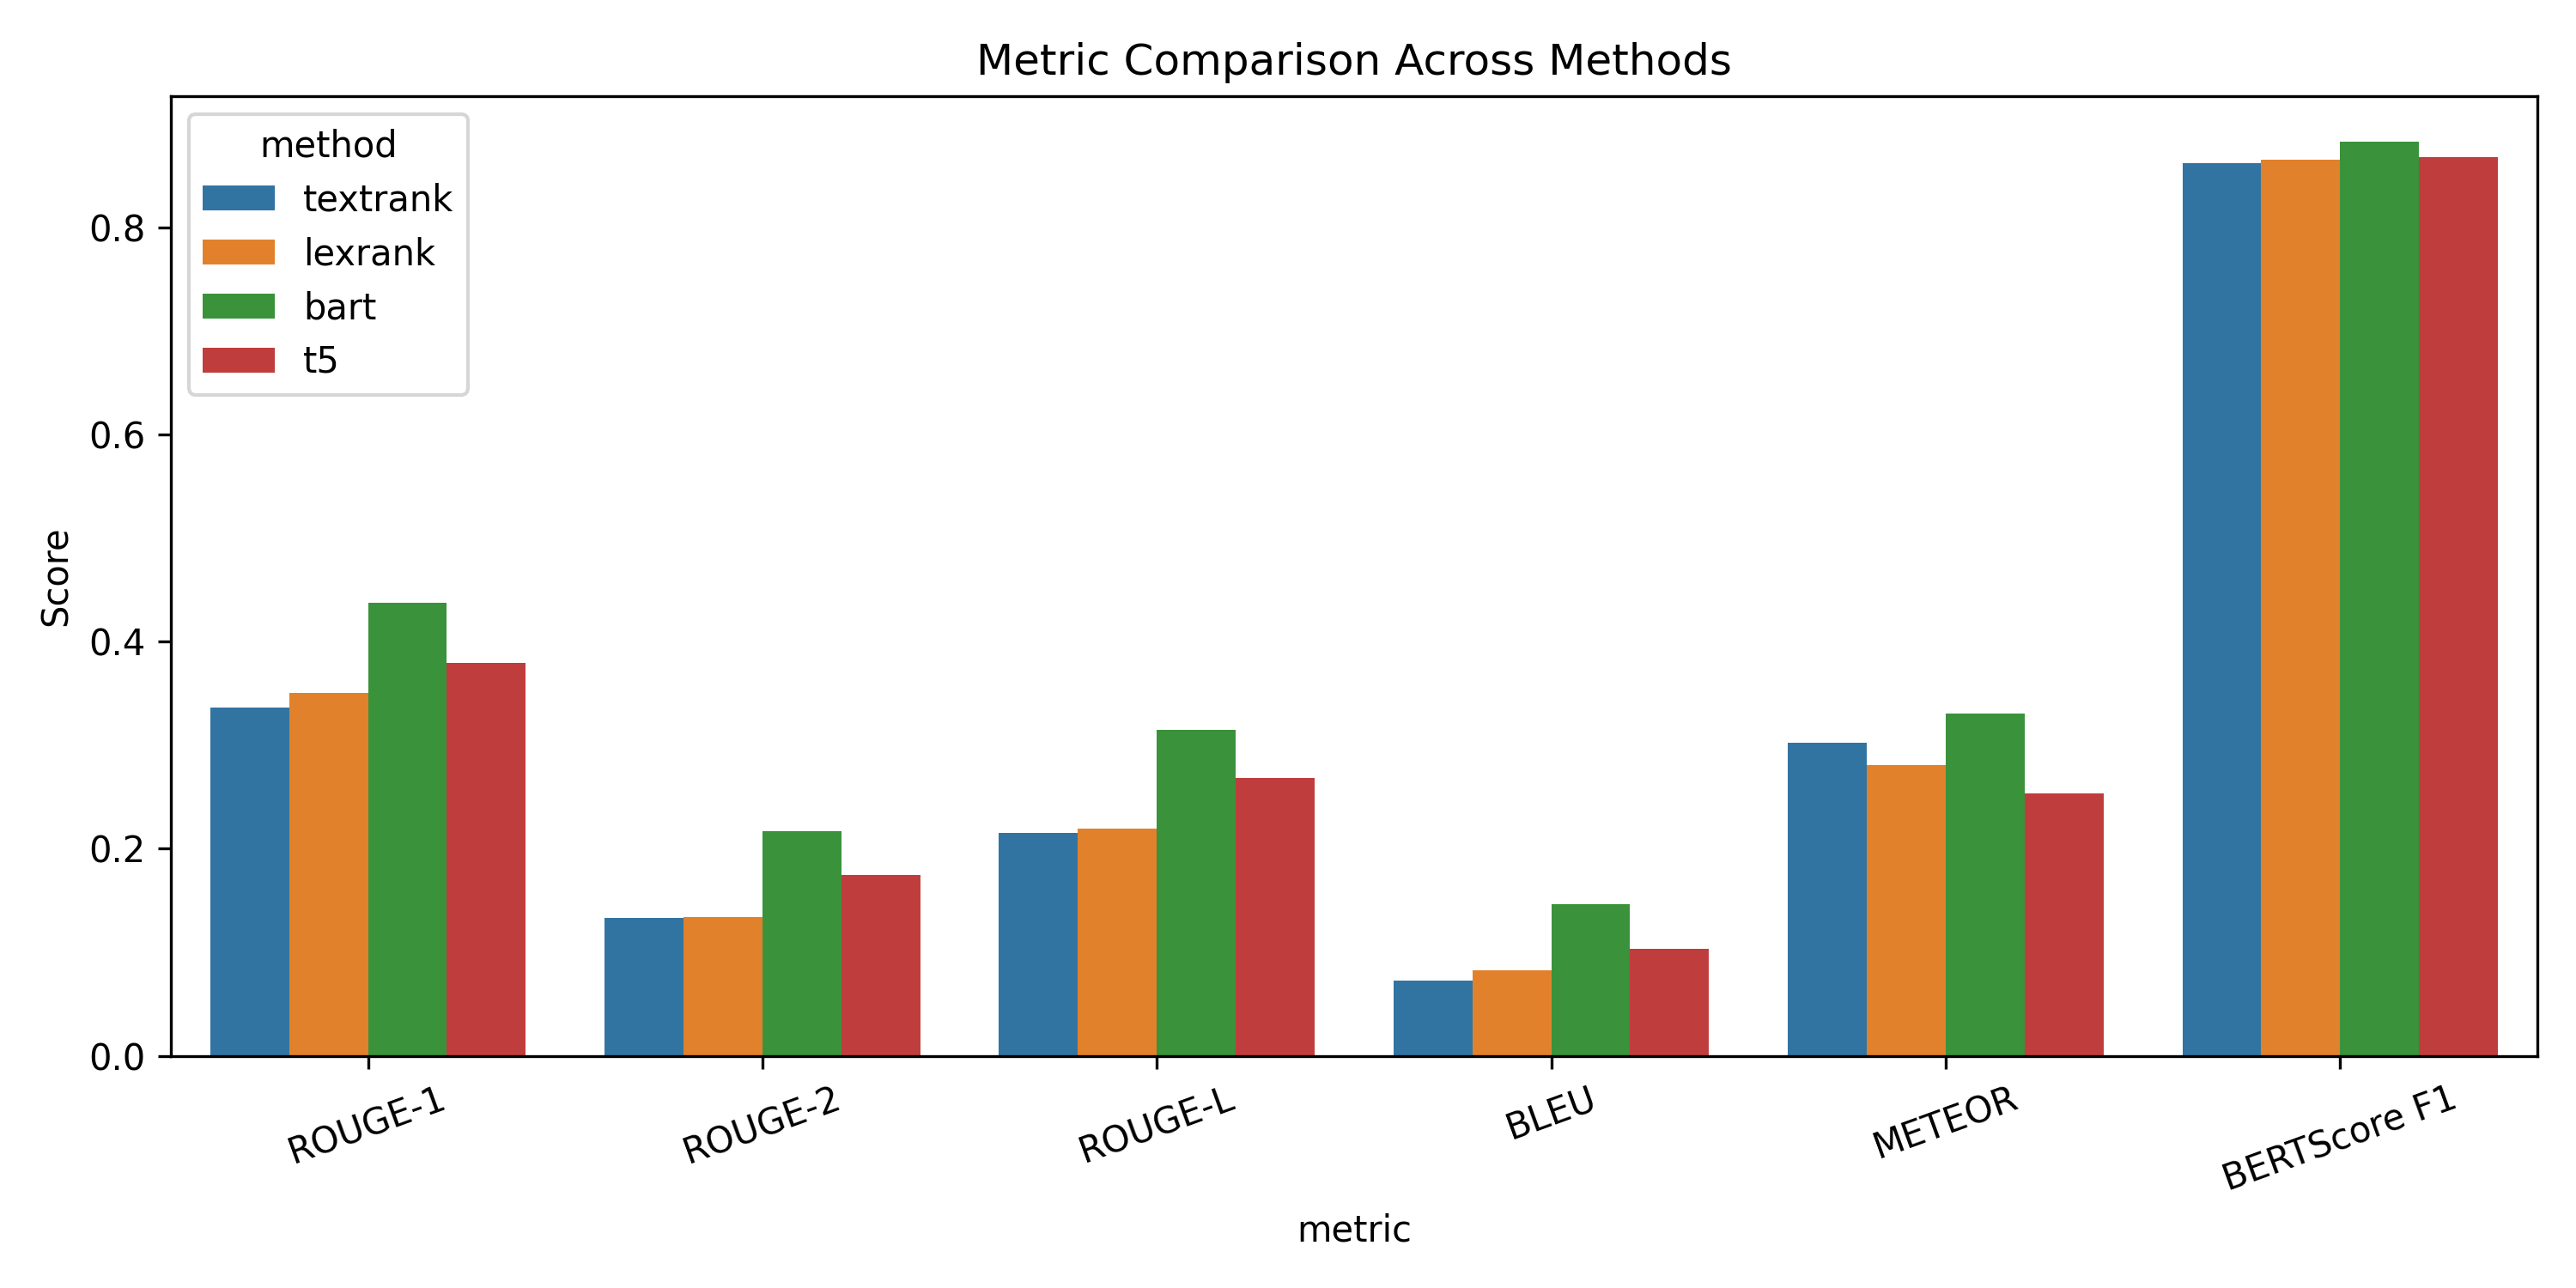
\includegraphics[width=0.90\linewidth]{../q3_summarization/outputs/figures/metric_comparison.png}
\caption{Metric comparison across all four methods.}
\end{figure}

\begin{figure}[H]
\centering
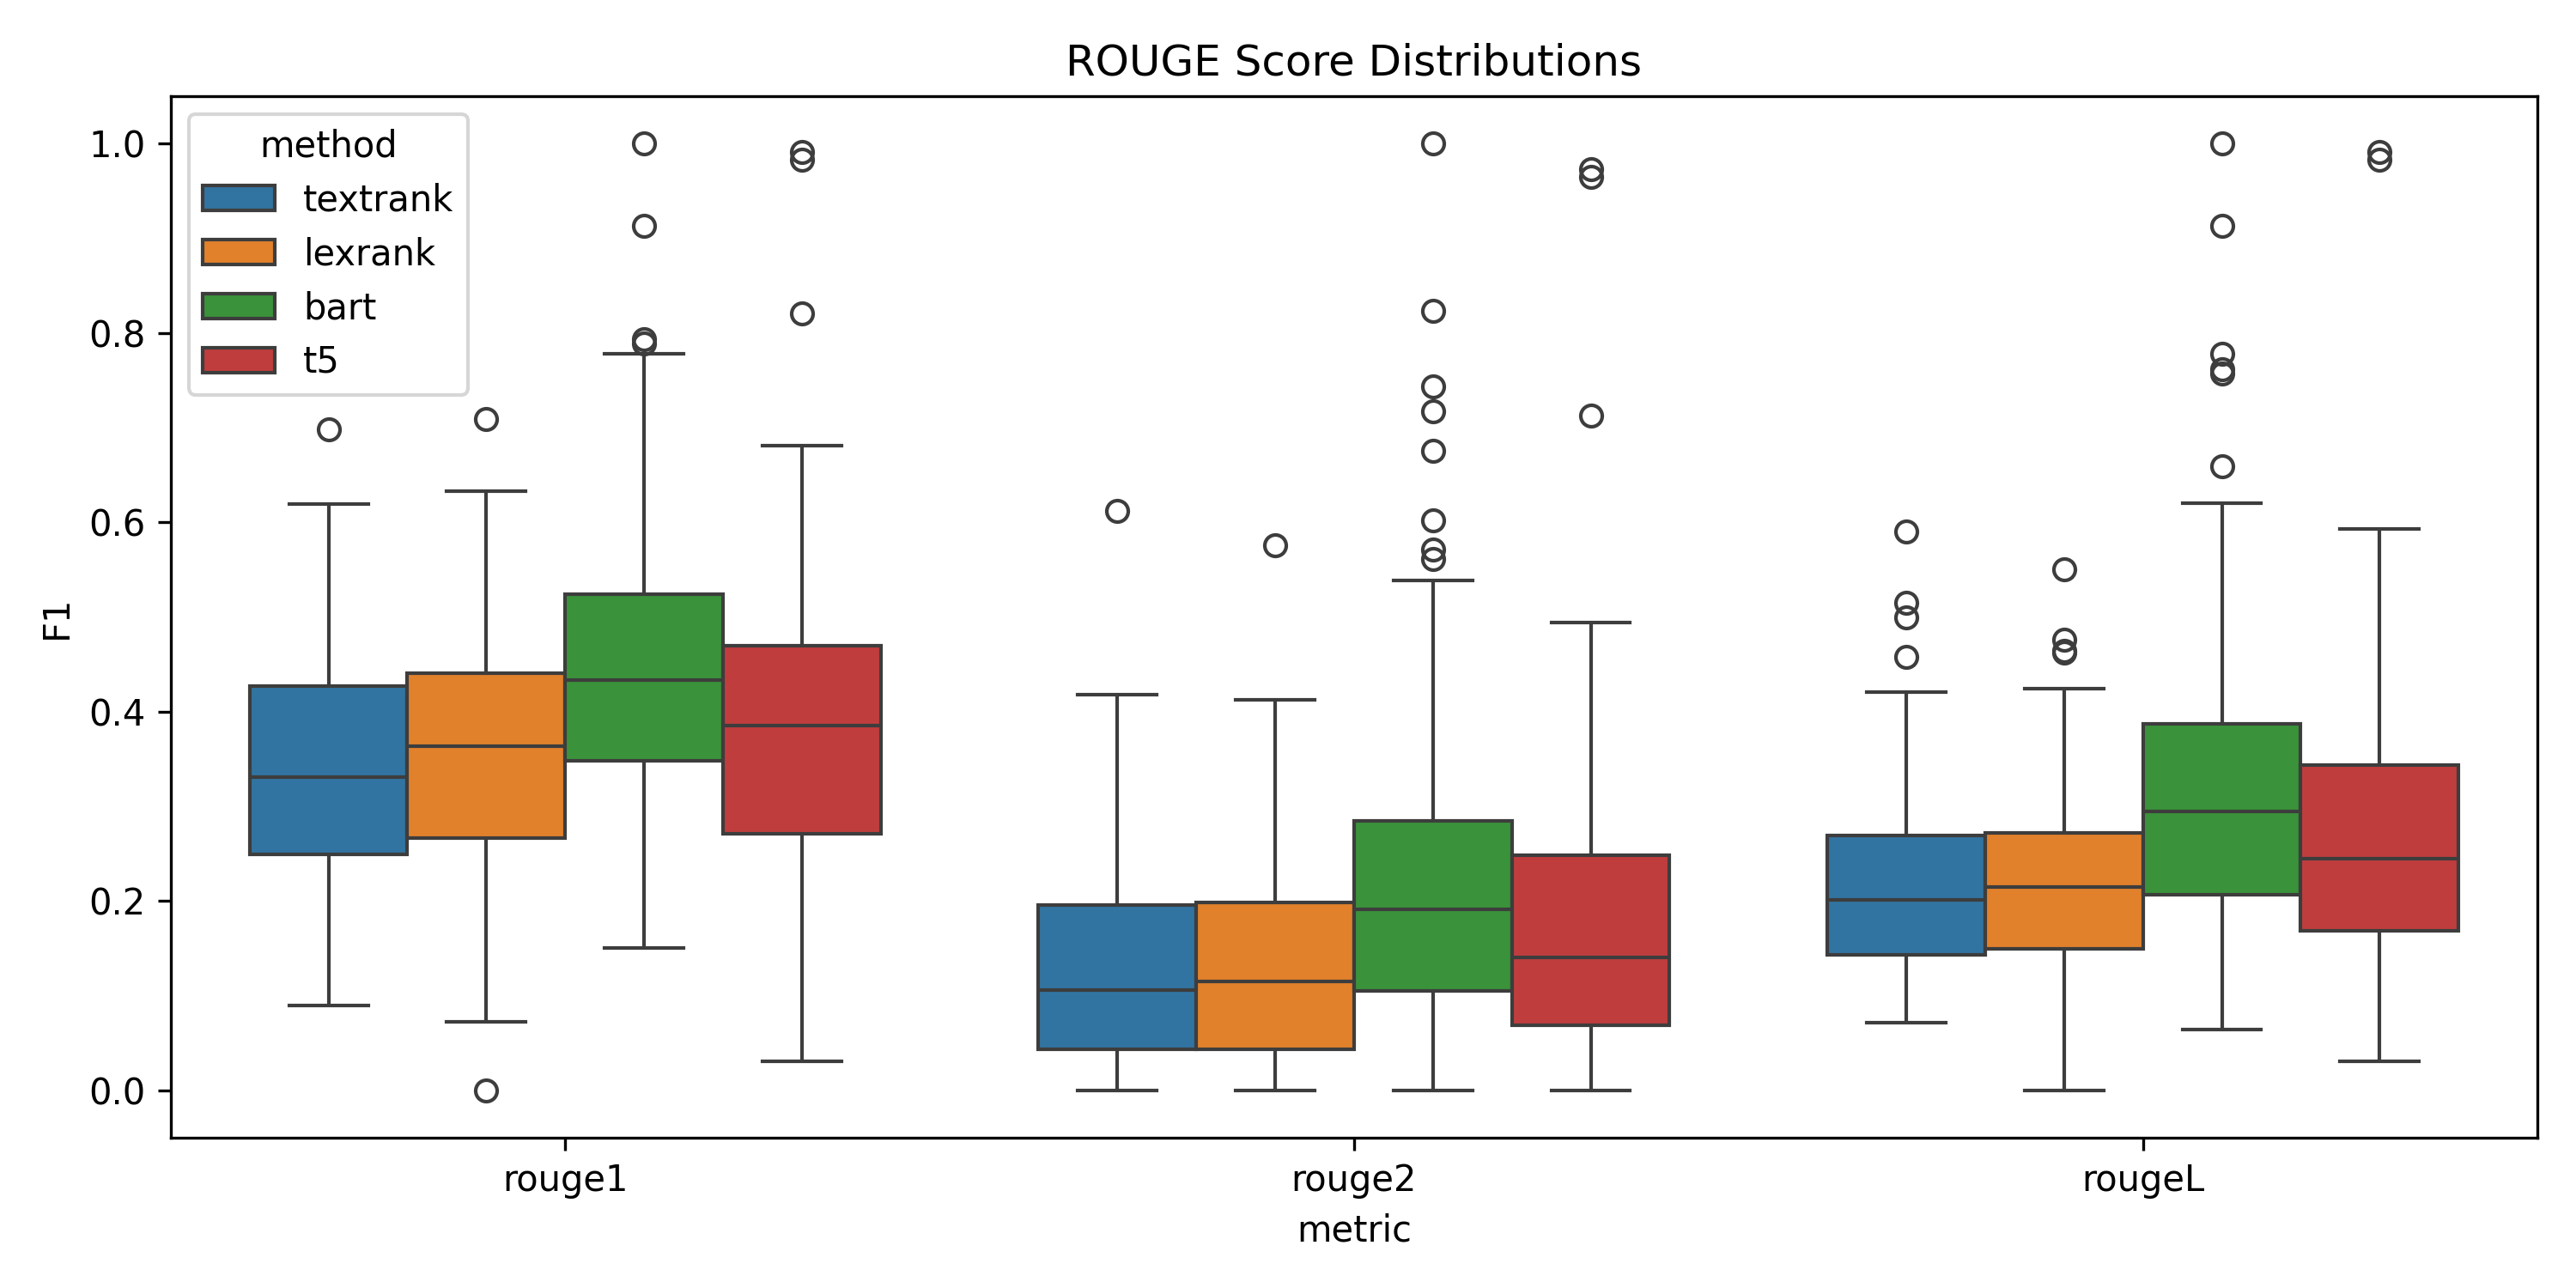
\includegraphics[width=0.90\linewidth]{../q3_summarization/outputs/figures/rouge_distributions.png}
\caption{ROUGE score distributions for each method.}
\end{figure}

\begin{figure}[H]
\centering
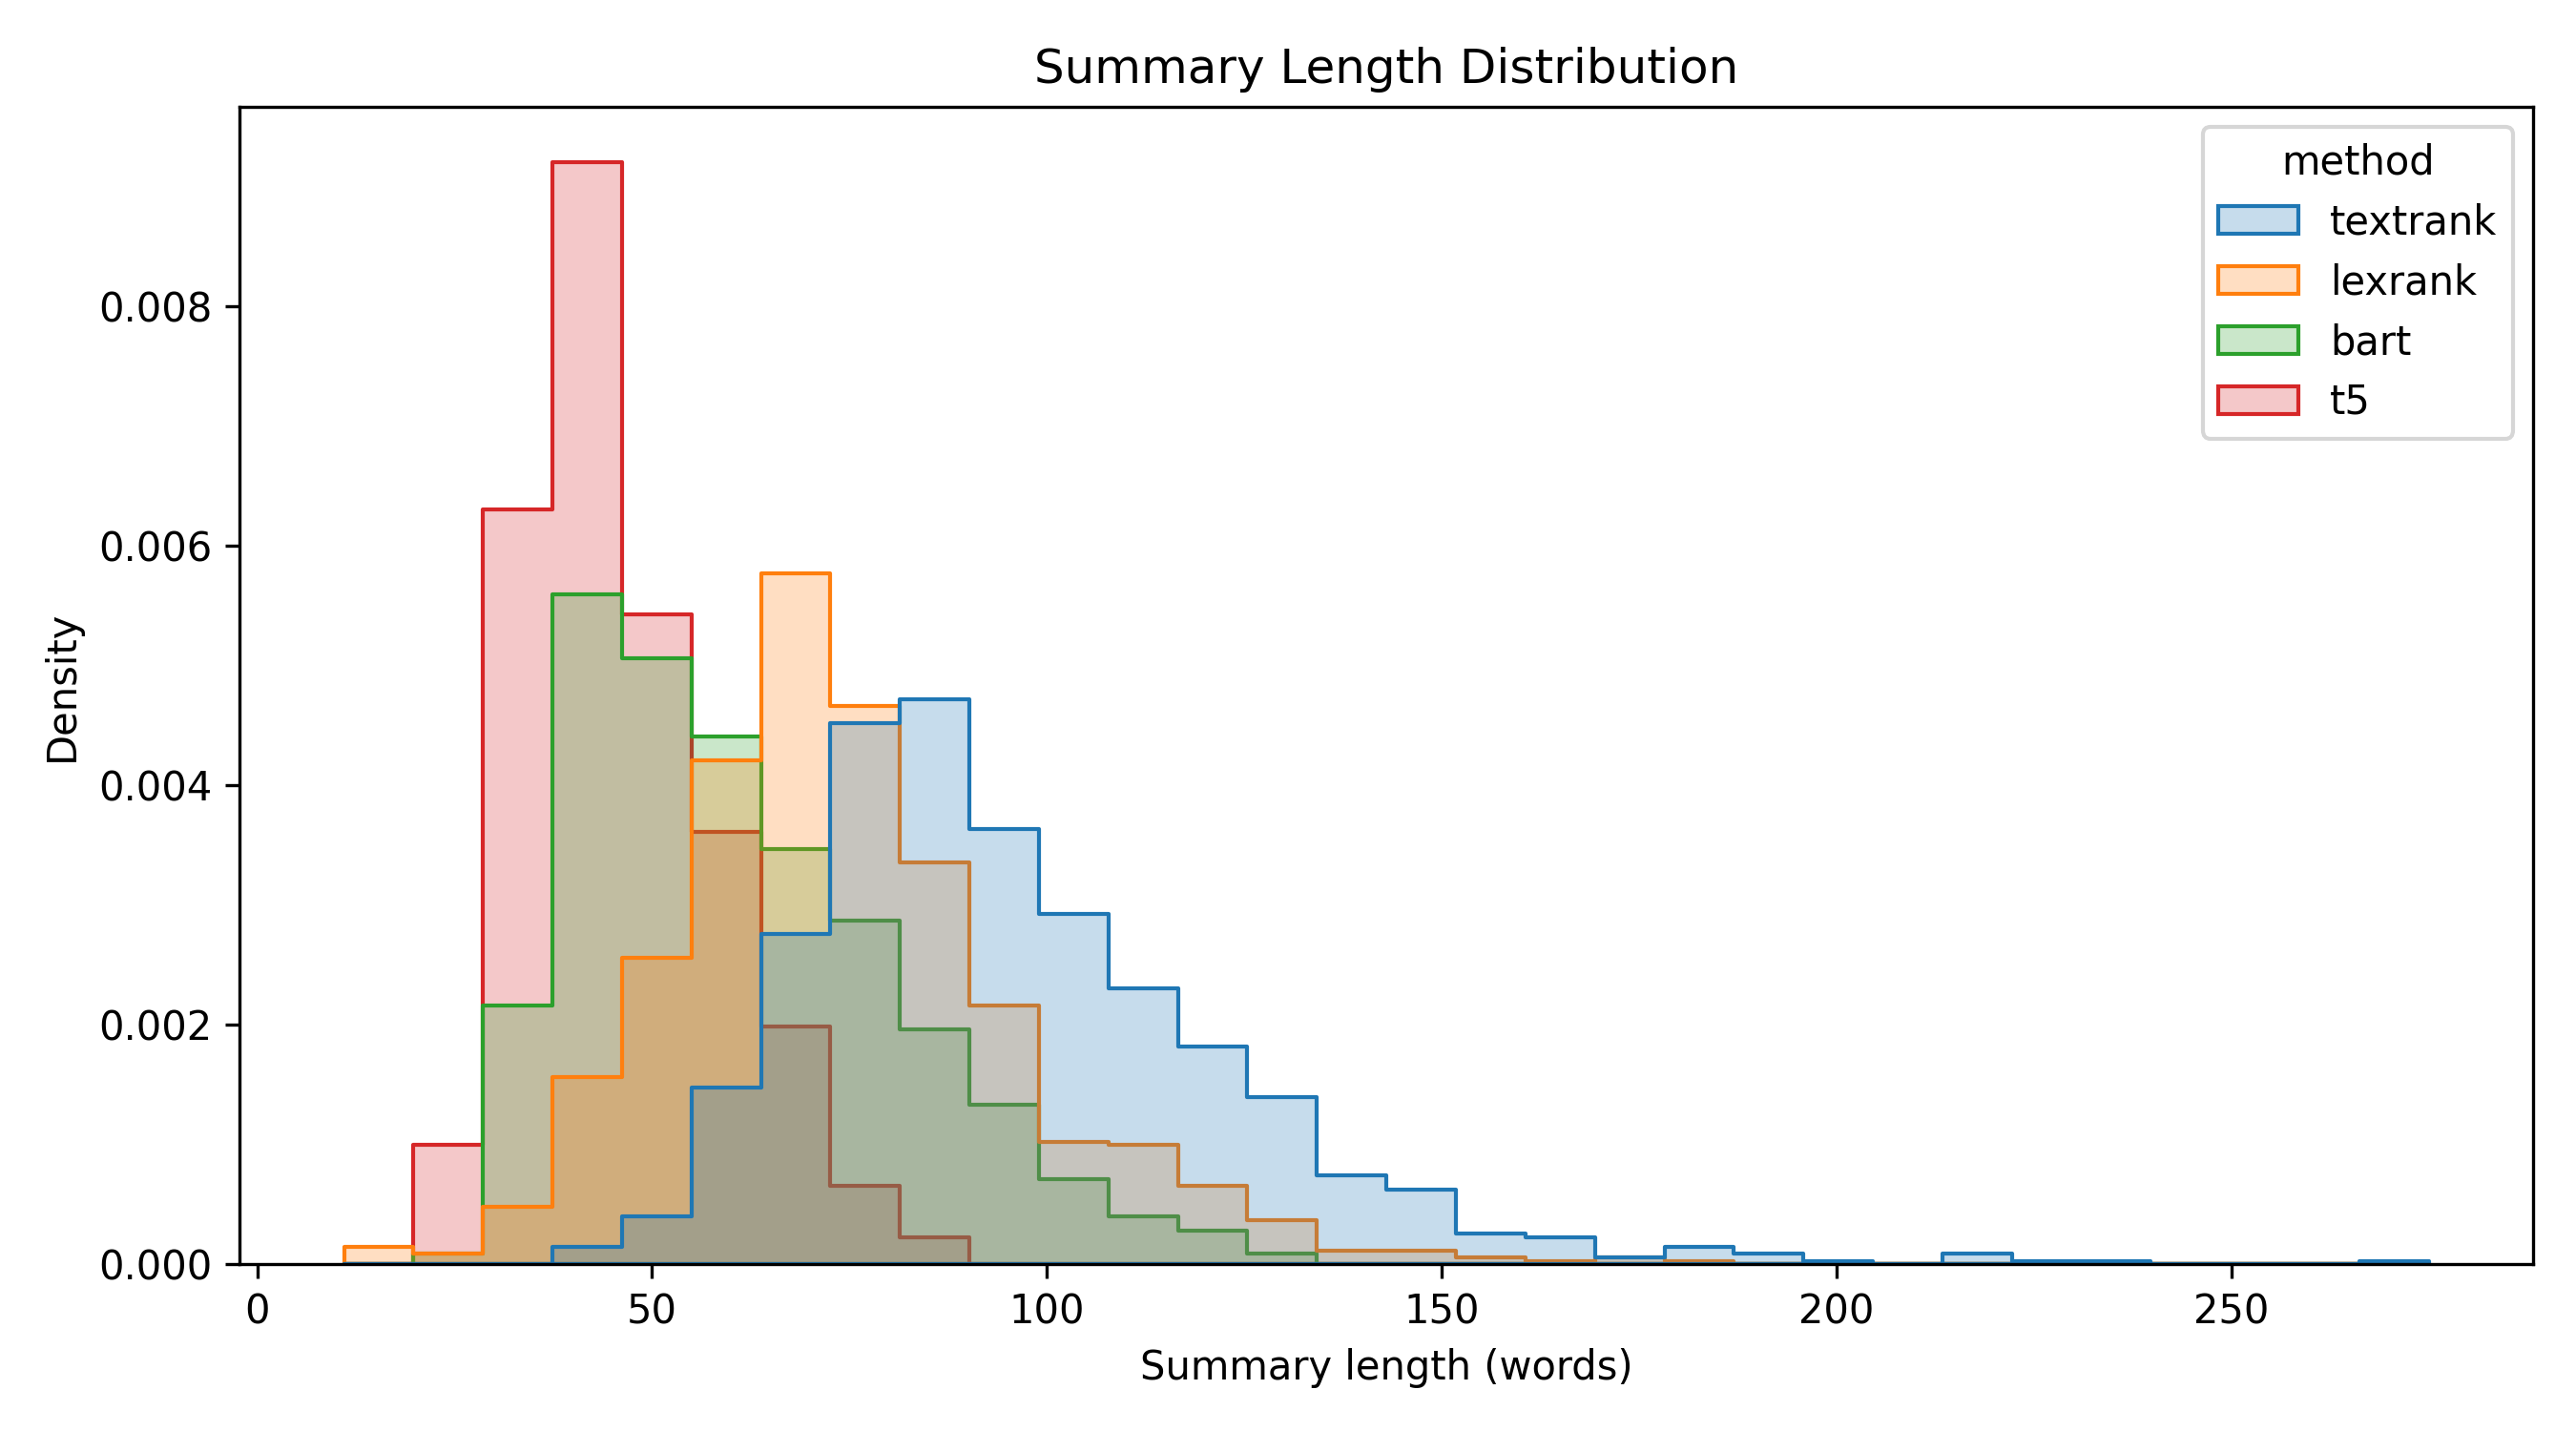
\includegraphics[width=0.85\linewidth]{../q3_summarization/outputs/figures/length_distribution.png}
\caption{Summary length distributions.}
\end{figure}

\begin{figure}[H]
\centering
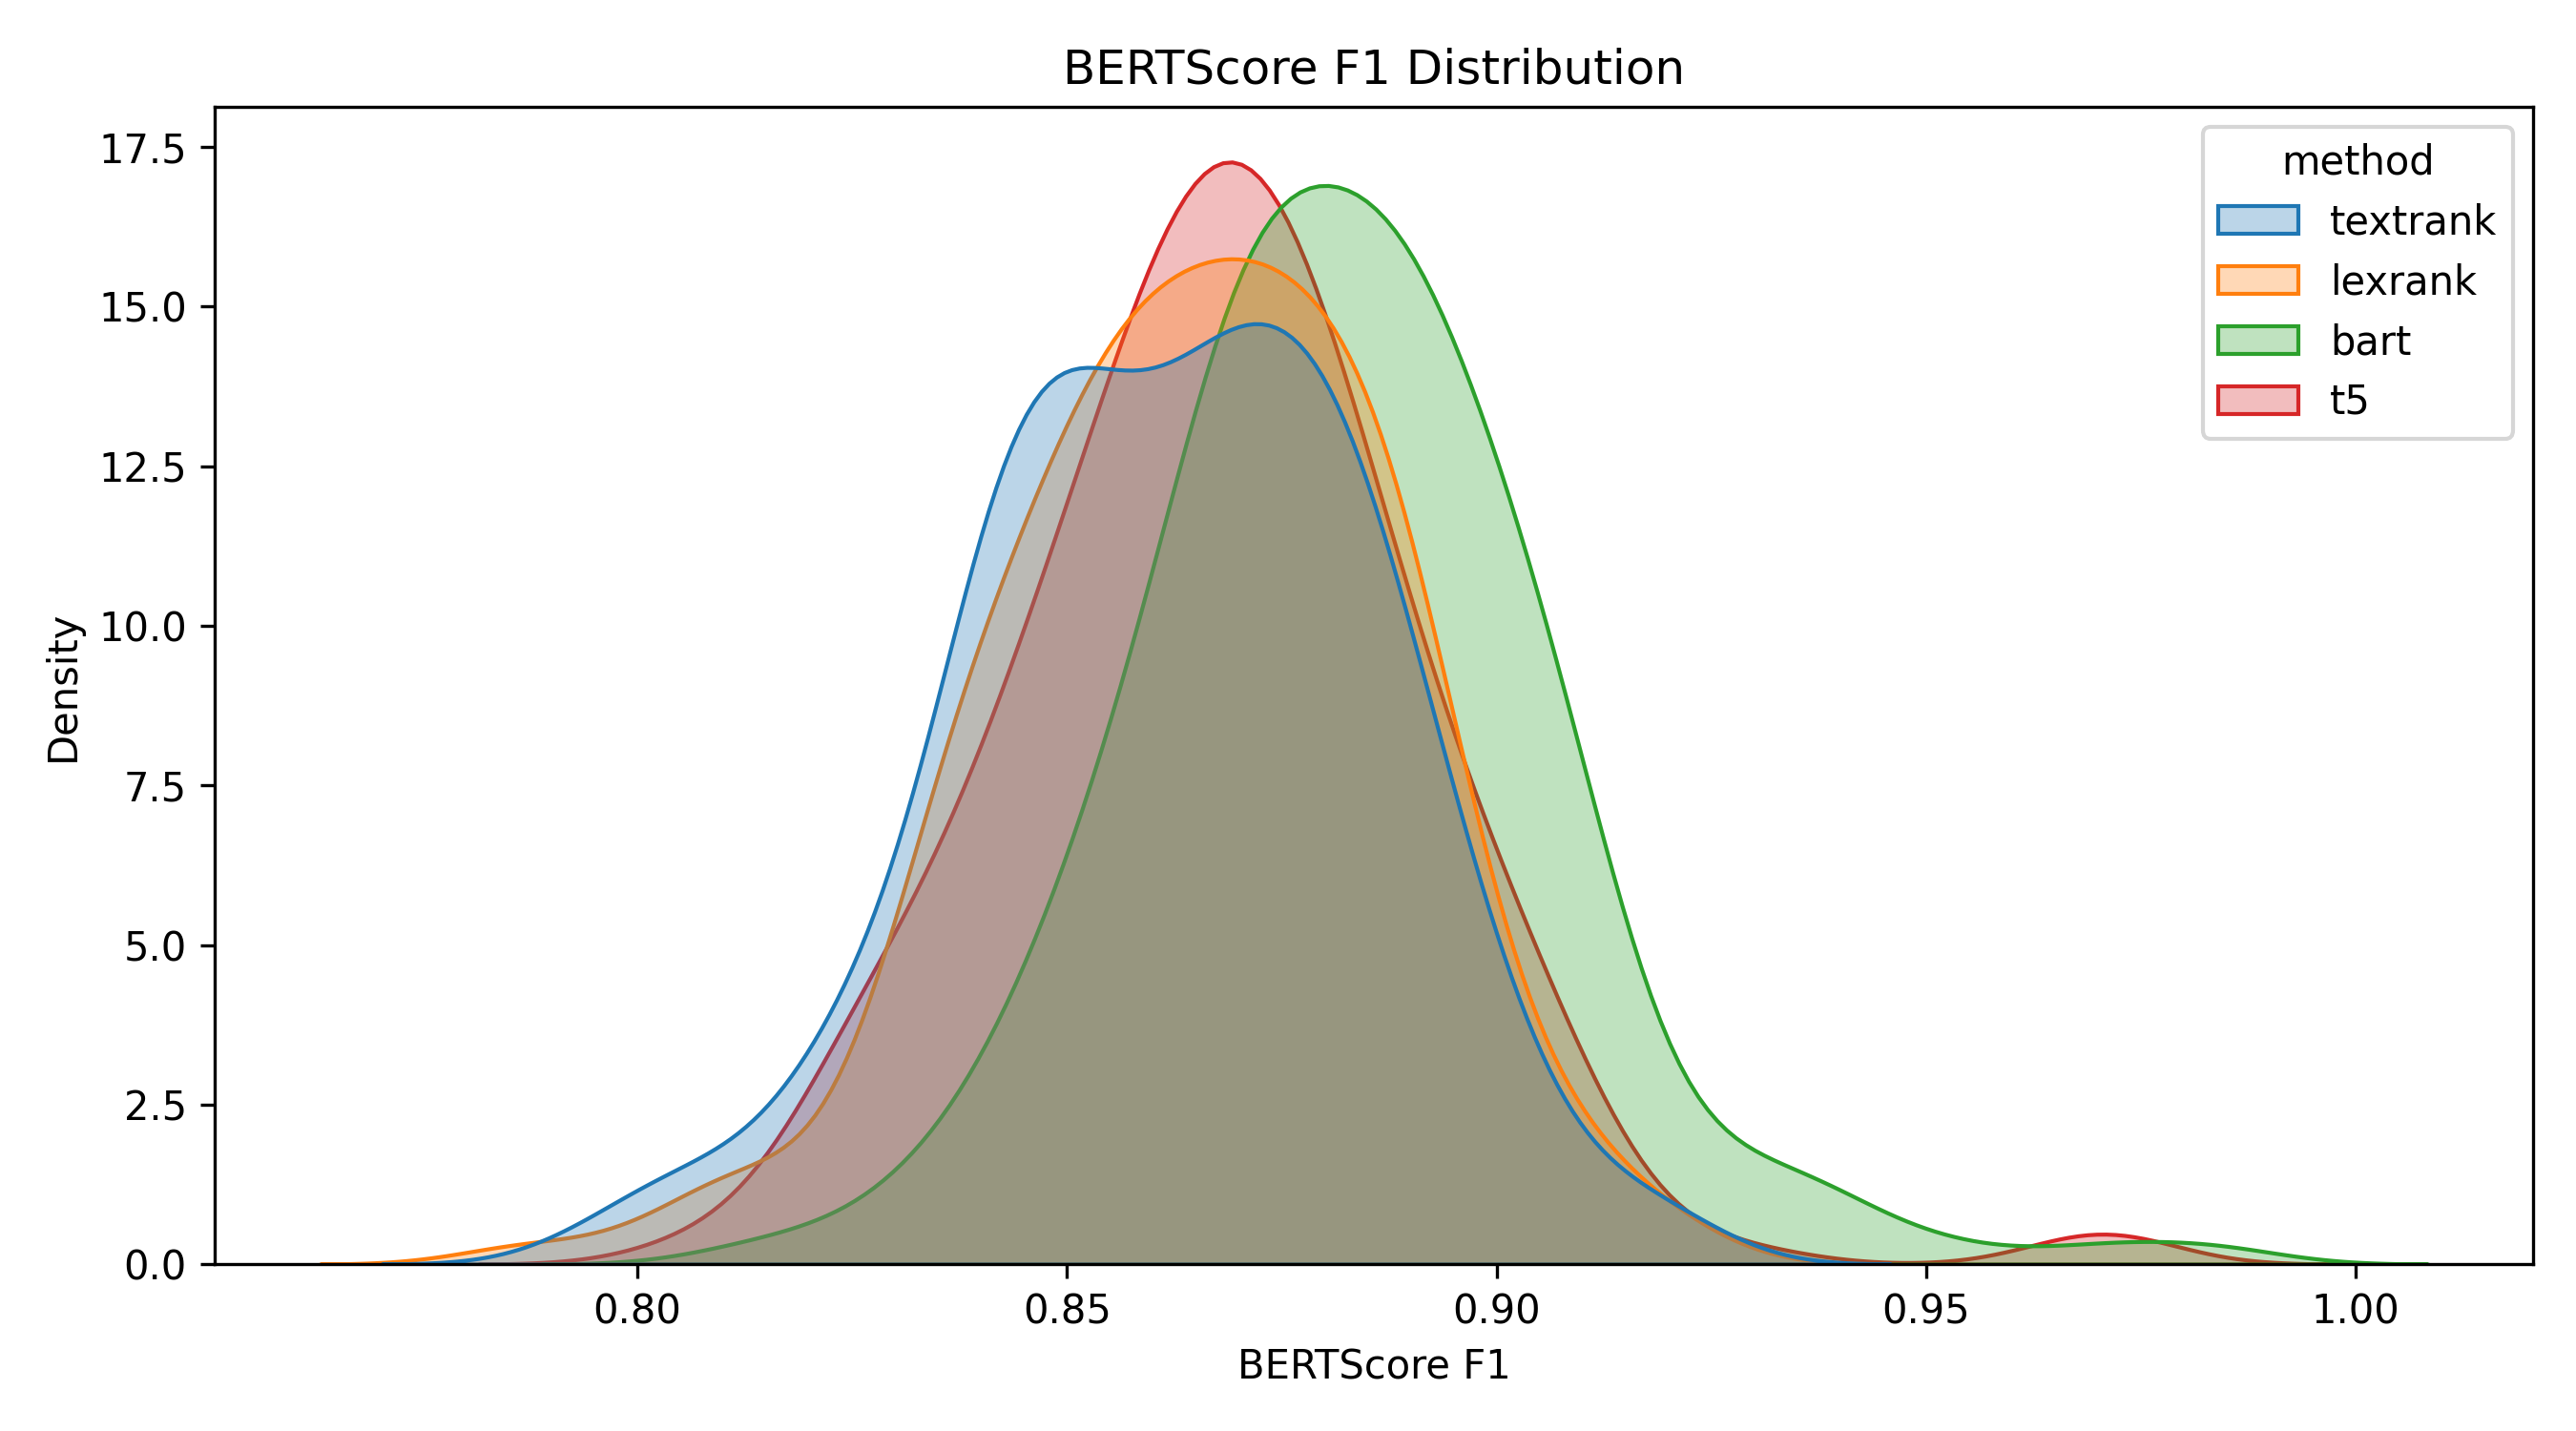
\includegraphics[width=0.85\linewidth]{../q3_summarization/outputs/figures/bertscore_distribution.png}
\caption{BERTScore F1 distributions.}
\end{figure}

\subsection{Qualitative Analysis}
We present three representative examples highlighting differences in fluency, faithfulness, and coverage. Text snippets are truncated for brevity.

\begin{table}[H]
\centering
\caption{Example 1 (extractive wins).}
\small
\begin{tabular}{p{0.18\linewidth} p{0.75\linewidth}}
\toprule
\textbf{Field} & \textbf{Text} \\
\midrule
Article & The legal adviser to Alison Saunders was a barrister in the same chambers as the son of Lord Janner... \\
Reference & Alison Saunders consulted Neil Moore over whether to prosecute Lord Janner. She said the decision was difficult and cited his health. \\
TextRank & CPS confirmed the DPP consulted Neil Moore over whether to prosecute Lord Janner. A spokesman said she decided alone. She said it was her job to make very difficult decisions. \\
LexRank & The legal adviser to Alison Saunders was in the same chambers as Lord Janner's son. A CPS spokesman said she decided alone. She admitted he should have been charged before. \\
BART & CPS confirmed the DPP consulted Neil Moore. Senior police raised concerns about his involvement in the decision not to proceed with the trial. \\
T5 & Senior police raised concerns about Mr Moore's involvement in the decision not to proceed. Mrs Saunders said she made the decision on her own. \\
\bottomrule
\end{tabular}
\end{table}

\begin{table}[H]
\centering
\caption{Example 2 (abstractive wins). Model outputs are quoted verbatim from \texttt{outputs/qualitative\_examples.json}; ``[\dots]'' marks elision for fit.}
\small
\begin{tabular}{p{0.16\linewidth} p{0.78\linewidth}}
\toprule
\textbf{Field} & \textbf{Text} \\
\midrule
Article & ``A British couple who are believed to have fled their Berkshire home with their four young children in a bid to escape to Syria have reportedly been arrested in Turkey. Asif Malik, 31, his partner Sara Kiran, 29, and their four children were caught on CCTV boarding a cross-Channel ferry from Dover [\dots] a Turkish official claimed today that the [family had been arrested in Ankara].'' \\
Reference & ``Asif Malik disappeared from UK with partner Sara Kiran and four children. Turkish official claimed today that the family have been arrested in Ankara. Malik, 31, was pictured holding `ISIS' sign at a protest in London last year. Relatives of Ms Kiran today made emotional appeal for her to come home.'' \\
TextRank & ``Malik and Ms Kiran, who neighbours said usually wore the full Islamic veil, left home without mentioning any holiday or travel plans [\dots] Both Malik and Dhar are believed to be followers of notorious preacher Anjem Choudary [\dots] Dhar -- one of Choudary's top henchmen -- fled to Syria with his pregnant wife and three young children last year while under investigation by Scotland Yard.'' \\
LexRank & ``A British couple who are believed to have fled their Berkshire home with their four young children in a bid to escape to Syria have reportedly been arrested in Turkey. The family of six have been missing from their home in Slough, Berkshire, since April 7. [\dots]'' \\
BART & ``Asif Malik, 31, his partner Sara Kiran, 29, and their four children were caught on CCTV boarding a cross-Channel ferry from Dover earlier this month. Thames Valley Police believed they arrived in Calais, France, before travelling south down through Europe in a bid to flee to Syria. But a Turkish official claimed today that the couple had been arrested in Ankara and are currently in custody. [\dots]'' \\
T5 & ``asif malik, 31, his partner Sara Kiran, 29, and their four children have reportedly been arrested in ankara. they were spotted boarding a cross-Channel ferry from dover earlier this month. [\dots] but a Turkish official claimed today that the couple had been arrested in ankara and are currently in custody with their four children.'' \\
\bottomrule
\end{tabular}
\end{table}

In Example~2 the abstractive systems clearly compress the article around the headline event (arrest in Ankara) and the cast of named entities, matching the reference's focus. The extractive systems pick up topically related but tangential material (Anjem Choudary, family veil) that inflates length without adding reference content. T5 lowercases proper nouns due to its sentence-level prefix-tuning training.

\begin{table}[H]
\centering
\caption{Example 3 (both struggle). Outputs verbatim from \texttt{outputs/qualitative\_examples.json}; ``[\dots]'' marks elision.}
\small
\begin{tabular}{p{0.16\linewidth} p{0.78\linewidth}}
\toprule
\textbf{Field} & \textbf{Text} \\
\midrule
Article & ``She may be a First Daughter, but Sasha Obama is still a teenager and can't seem to tear herself away from her music -- even for a rare family nature hike. Sasha, 14, was spotted listening to earbuds [\dots] for an impromptu trip to Great Falls Park in Virginia on Sunday. The unscheduled trip came after the White House had sent reporters home for the day [\dots]'' \\
Reference & ``President Obama abruptly left the White House after reporters were sent home for the day Sunday evening. Press pool reporters were perplexed as they questioned whether something serious had happened. The president, Michelle and their girls hiked through Great Falls Park in Virginia for around 50 minutes until a light rain sent them packing.'' \\
TextRank & ``Tuning out of politics: Sasha Obama, 14, was spotted with white earbuds [\dots] Gorgeous; Great Falls Park is a National Park located in Virginia [\dots] The family's brief hike happened to take place during the National Park Service's National Park Week. President Obama, First Lady Michelle Obama (not seen) and their daughters Malia (3rd L) and Sasha (C) return from a hike at Great Falls National Park in Virginia as rains began to fall Sunday evening.'' \\
LexRank & ``Sasha, 14, was spotted listening to earbuds [\dots] for an impromptu trip to Great Falls Park in Virginia on Sunday. Took a hike: The Obamas abruptly left the White House for an unscheduled family nature hike on Sunday. President Obama, First Lady Michelle Obama (not seen) and their daughters Malia (3rd L) and Sasha (C) return from a hike at Great Falls National Park in Virginia as rains began to fall Sunday evening.'' \\
BART & ``Sasha, 14, was spotted listening to earbuds as she, sister Malia and their parents ditched the White House -- and the press pool -- for an impromptu trip to Great Falls Park in Virginia on Sunday. The family's brief hike happened to take place during the National Park Service's National Park Week. \textbf{On Saturday, Obama spent his Saturday afternoon golfing at Joint Base Andrews.}'' \\
T5 & ```obama abruptly left the White House about 15 minutes ago on unscheduled trip. Destination unknown,' tweeted Byron Tau. reports initially seemed to fear that the unscheduled departure was some sort of emergency [\dots] the family's brief hike happened to take place during the National Park Service's National Park Week.'' \\
\bottomrule
\end{tabular}
\end{table}

In Example~3 every system misses at least one reference fact. Both extractive systems return long photo-caption sentences that the reference does not include. BART's last sentence (bolded) is an extrinsic hallucination -- the article does not mention golfing on Saturday or Joint Base Andrews. T5 is more faithful but omits the ``50 minutes'' and ``light rain'' timeline that the reference centres on. ROUGE penalises all four systems here even though the lexical overlap with the source is high; this is a typical failure mode where the reference is itself an aggressive paraphrase.

\subsection{Discussion: Trade-offs}
Abstractive models (especially BART) achieve the strongest ROUGE and BERTScore, and their summaries are more concise and readable. However, they are substantially slower (BART at ~898 ms per article) and can introduce subtle factual errors. Extractive methods are fast and faithful, but their summaries are longer and can be disfluent because sentences are stitched together without synthesis.

\textbf{Metric limitations.} ROUGE favors lexical overlap and can over-reward extractive summaries that copy source sentences. Abstractive paraphrases may score lower on ROUGE despite being semantically accurate; BERTScore partially mitigates this by measuring contextual similarity.
